\section{Problem I}
\textbf{solution}:\\
According to the description above, this problem could be mapped to a single source Directed acyclic graph(DAG) as follows:
\begin{itemize}
	\item Corridors $\rightarrow$ directed edge
	\item Elevators $\rightarrow$ directed edge
	\item Food Location $\rightarrow$ vertex
	\item Exit Point $\rightarrow$ vertex
	\item Entry Point $\rightarrow$ vertex source
	\item Food Quantity $\rightarrow$ weight on vertex
\end{itemize}

So, the input of this problem is a DAG denoted as $G(V, E)$. And the quantity of food at food location could also be described as the weight on every edge directed to the corresponding food location(vertex). The output should be a path $P$ in $G$ that accumulate the max gain(food) across all paths in $G$ from $S$ to any vertex.

\begin{figure}[h]
\centering
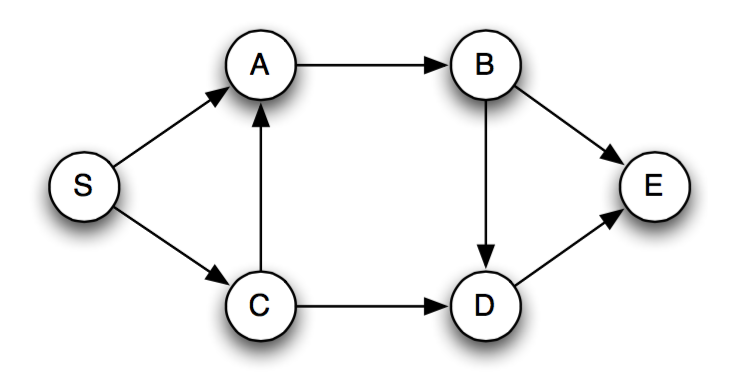
\includegraphics[scale=0.4]{DAG}
\caption{A DAG example mapped from problem}
\label{fig:p1}
\end{figure}

For example, suppose we have a DAG as shown in Figure \ref{fig:p1}. We could traverse the vertices in linearized order from left to right since a DAG can always be topologically sorted or linearized. As shown in Figure \ref{fig:p2}, we the linearized version of the DAG shown in Figure \ref{fig:p1} are then: $\left\{S, C, A, B, D, E\right\}$. 

\begin{figure}[h]
\centering
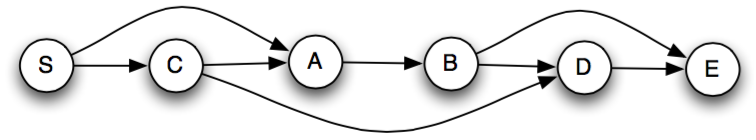
\includegraphics[scale=0.4]{lineardag}
\caption{Linearized version of $G$}
\label{fig:p2}
\end{figure}

The problem equivalent to find the longest path from vertex $S$ to any other vertex. Consider the vertex $D$ in the linearized graph - the only way to get to $D$ from $S$ is through one of its predecessors: $B$ and $C$. That means, to compute the longest path from $S$ to $D$, one must first compute the longest path from $S$ to B (up to the first predecessor), and the longest path from $S$ to $C$ (up to the second predecessor). Once we've computed the longest paths from $S$ to these two predecessors, we can compute the longest path to $D$ by taking the larger of these two, and adding $w(D)$(food quantity in $D$). If $dist(v)$ is the longest distance from $S$ to vertex $v$, and $\alpha(v)$ is the actual path, then we can write the following recurrence for $dist(D)$:

$$ dist(D) = max\left\{ dist(B) + w(D), dist(C) + w(D) \right\} $$

Note the subproblems here: $dist(B)$ and $dist(C)$, both of which are “smaller” than $dist(D)$. Similarly, we can write the recurrences for $dist(B)$ and $dist(C)$ in terms of its subproblems:

$$ dist(B) = dist(A) + w(B) $$
$$ dist(C) = dist(S) + w(A) $$

For the source vertex $S$, we set:

$$ dist(S) = w(S) $$
$$ \alpha(S = \left\{ S \right\} $$

We are now ready to write the recurrence for the longest path from $S$ to any other vertex $v$ in $G$, which involves first computing the longest paths to all of $v$'s predecessors from $S$ (these are the subproblems).

$$ dist(v) = max_{(u, v) \in E}{dist(u) + w(v)} $$

And, we can compute this bottom-up for each vertex $v \in V$ taken in a linearized order. The final algorithm is shown below:\\

LONGEST-PATH($G$)\\
Input: Weighted DAG $G$\\
Output: Largest path cost in $G$\\
Topologically sort $G$\\
\textbf{for} each vertex $v \in V$ in linearized order\\
\hspace*{0.6cm} \textbf{do}:\\
\hspace*{0.6cm} dist($v$) $\gets$ $\text{max}_{(u, v) \in E}\left\{ \text{dist}(u) + w(v) \right\}$\\
\hspace*{0.6cm} $\alpha(v) \gets \text{max}_{(u, v) \in E}\left\{ \alpha(u) \cup v \right\}$\\
\textbf{return} $\text{max}_{v \in V} \left\{ \text{dist}(v) \right\}$\\

The time complexity is obvious $O(\mid V \mid + \mid E \mid)$.

